\newpage

\section{Capas}

He dividido los componentes de la grúa en 3 capas:

\begin{itemize}
    \item \textbf{Controladores: }Esta capa almacena los \textit{sliders} que controlan el movimiento de la excavadora y los controladores de los huesos.
    
    % foto de eso
    \begin{figure}[H]
        \centering
        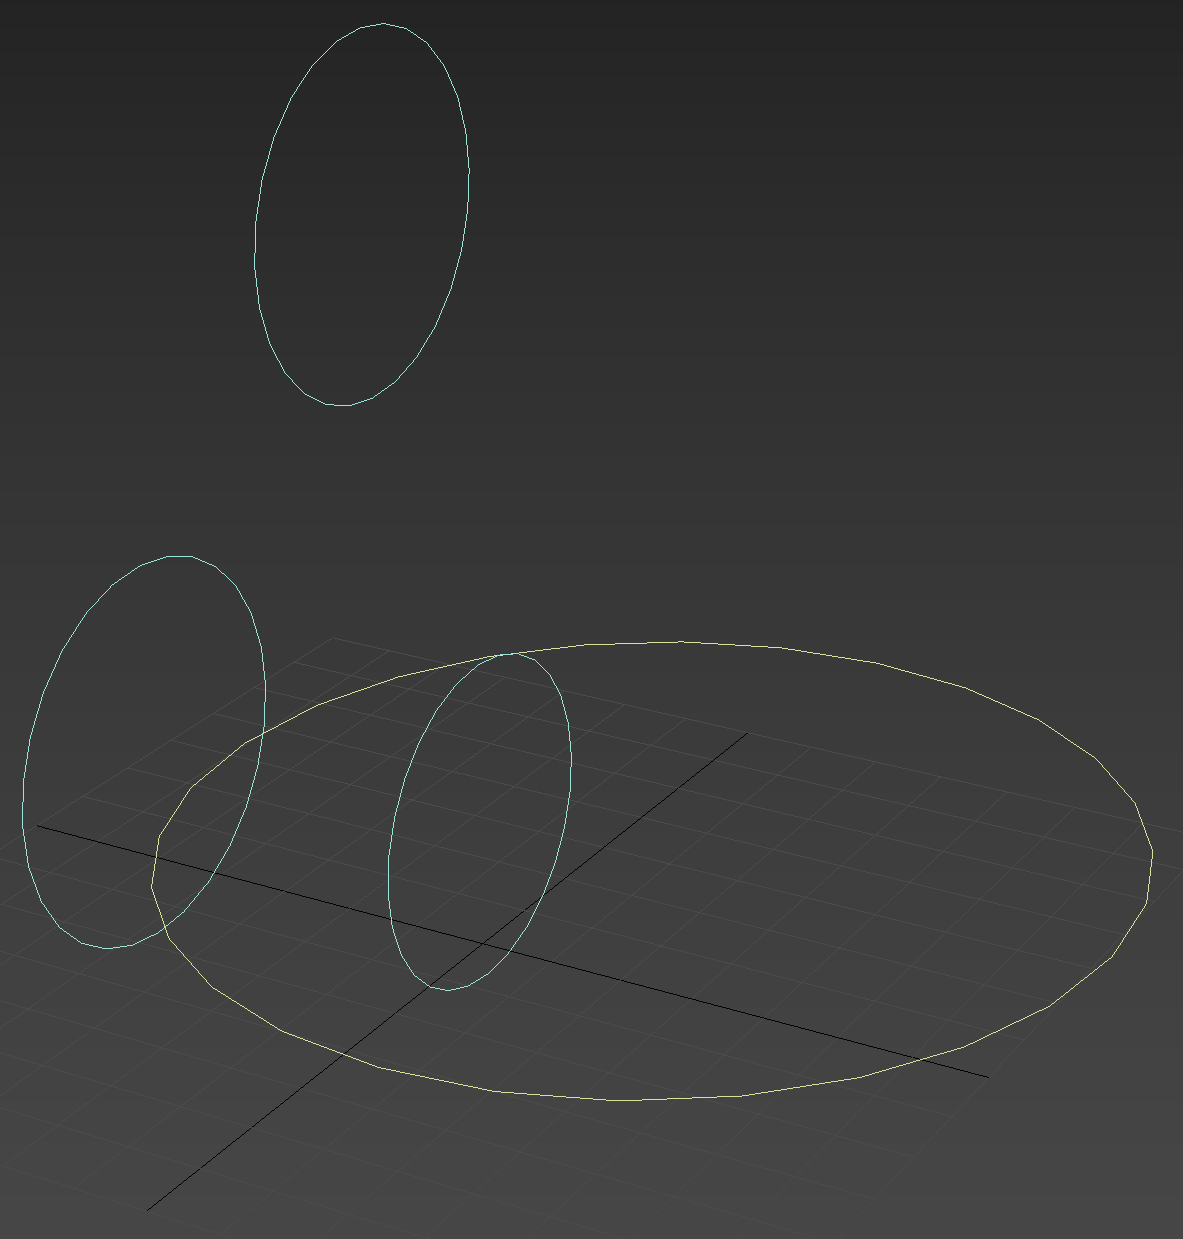
\includegraphics[width=0.4\textwidth]{imagenes/controladorcapa.png}
        \caption{Vista de la capa de controladores.}
     \end{figure}

    \item \textbf{Esqueleto: }No habría sido necesario en esta figura, pero he decidí usarlos en una etapa muy temprana y ya es muy complicado cambiarlo.
    
    Los huesos de la excavadora son:


    % foto de los huesos
    \begin{figure}[H]
        \centering
        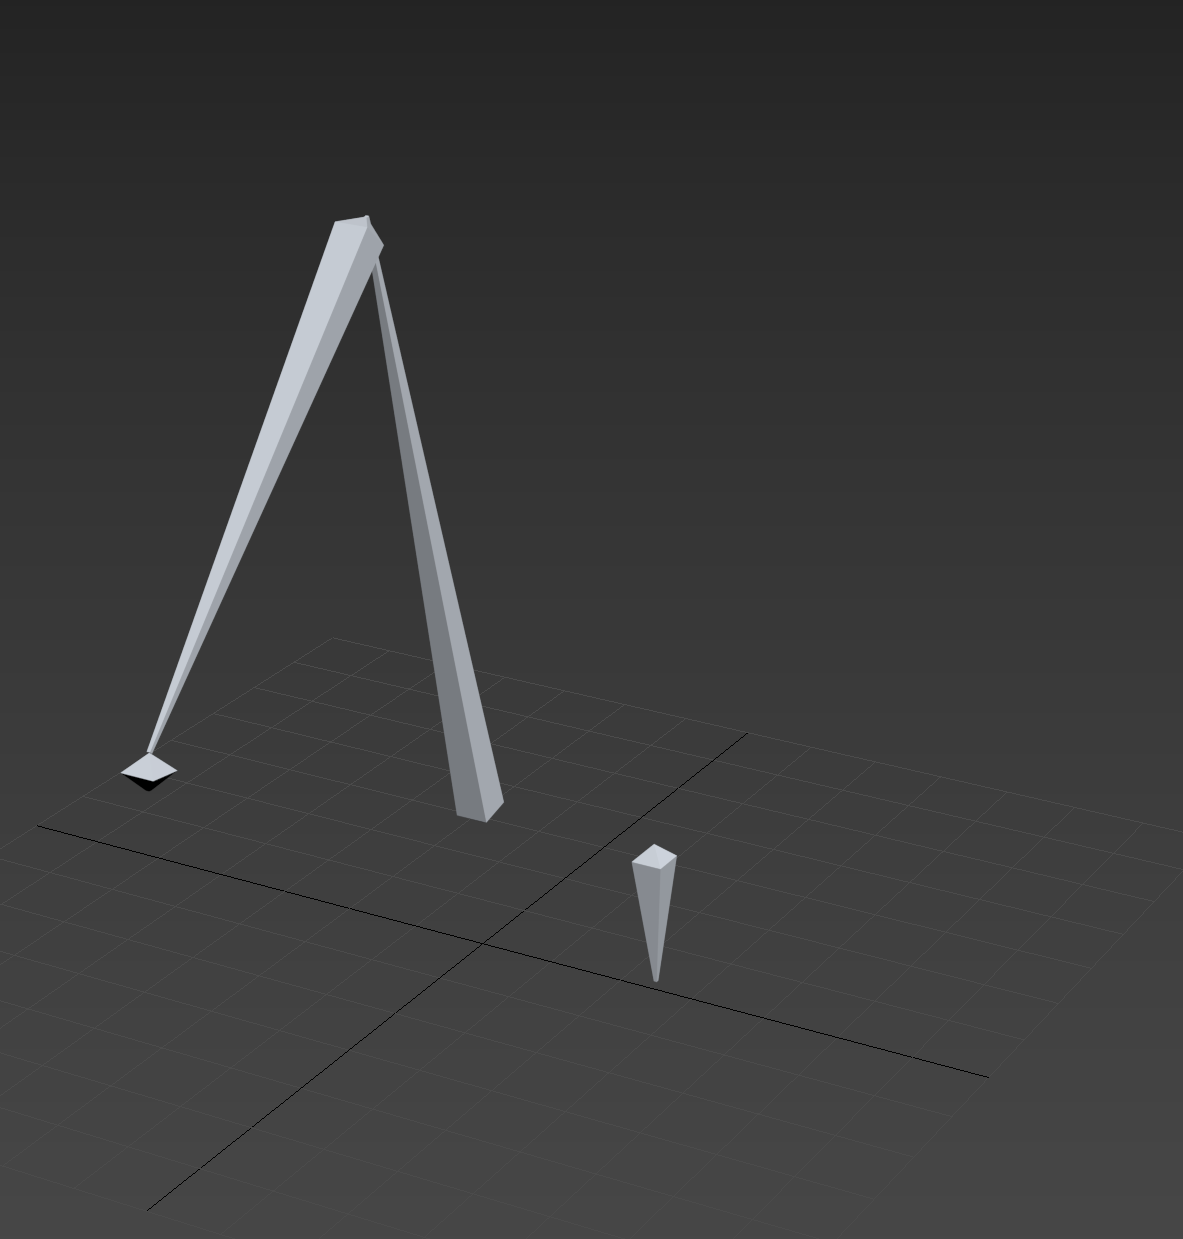
\includegraphics[width=0.4\textwidth]{imagenes/esqueletocapa.png}
        \caption{Vista de la capa del esqueleto.}
     \end{figure}

    Como se puede ver, tiene un hueso debajo que es el que se encarga de mover toda la cabina y el brazo. Después, tiene los huesos del propio brazo.

    \newpage

    \item \textbf{Modelo: }Esta capa es la utilizada para almacenar el modelo de la excavadora.
    
    % foto de la capa
    \begin{figure}[H]
        \centering
        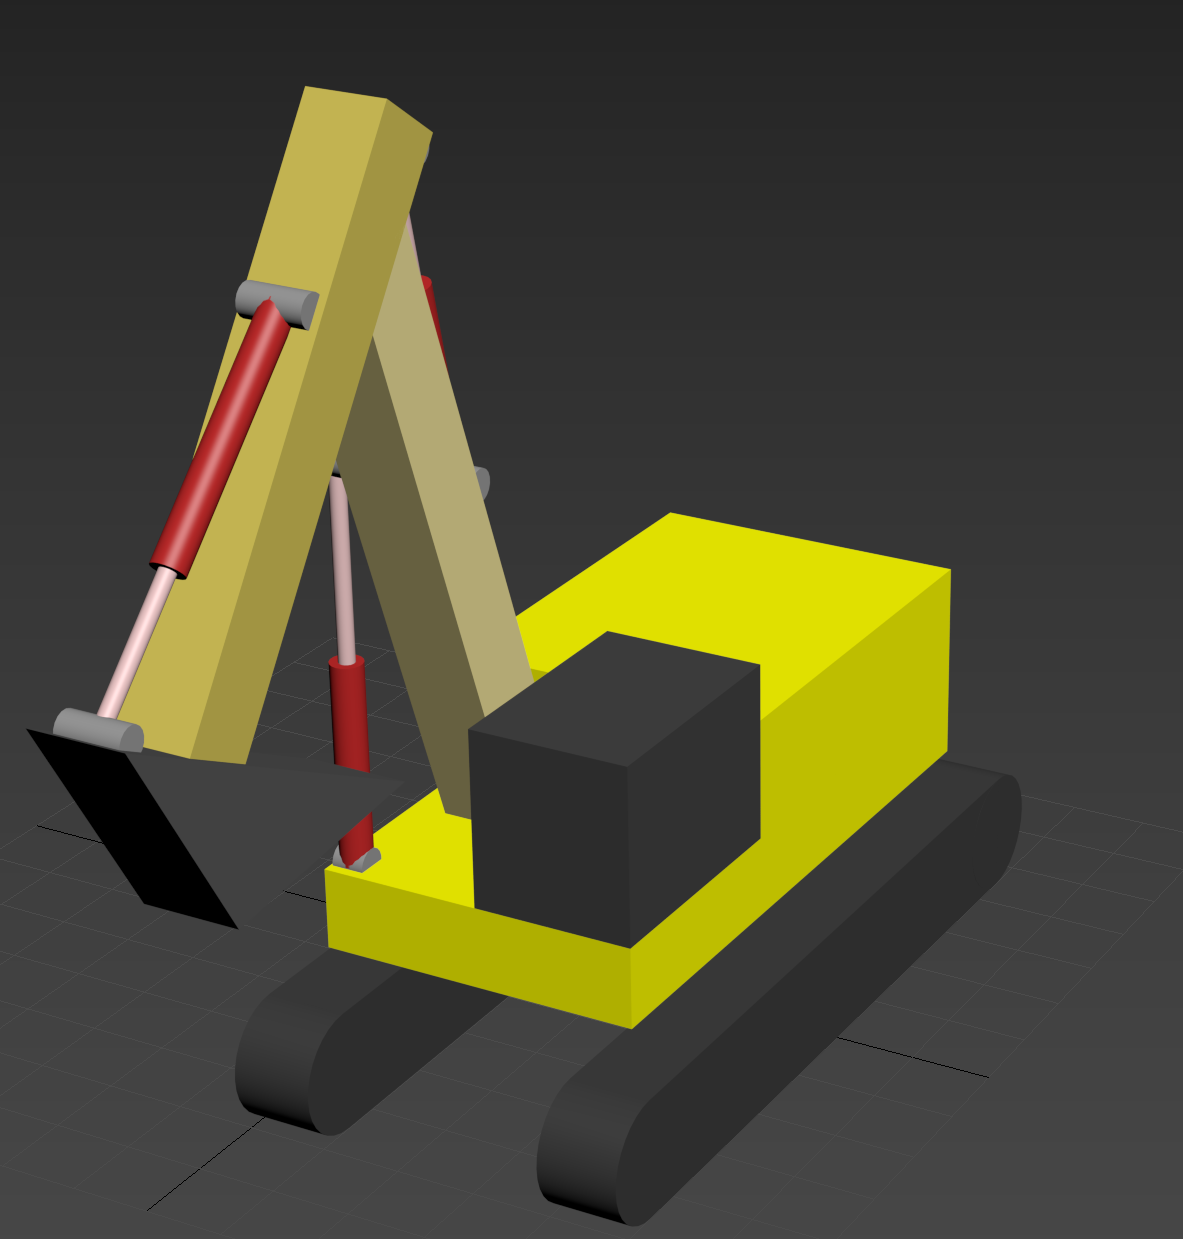
\includegraphics[width=0.4\textwidth]{imagenes/modelocapa.png}
        \caption{Vista de la capa del modelo.}
     \end{figure}
\end{itemize}